% =============================================================================
% ch05_fusion.tex : Chapter 5: Sensor Fusion Architecture
% =============================================================================
\selectlanguage{hebrew}

\section{ארכיטקטורת מיזוג חיישנים}
\label{sec:sensor_fusion}

מיזוג רב-חיישנים הוא חיוני לניווט תת-ימי חזק, שכן אף חיישן בודד אינו מספק מדידות אמינות בכל תנאי ההפעלה. בפרק זה נציג את ארכיטקטורת מיזוג החיישנים ההדוק (\en{tightly-coupled fusion}) המבוססת על גרף גורמים, המשלבת מדידות מ-\en{IMU}, \en{DVL} וסונאר במסגרת אחידה. \citet{Thrun2005ProbRobotics} הניחו את היסודות התאורטיים למיזוג רב-חיישנים במערכות \en{SLAM}, תוך הדגשת החשיבות של מודלים הסתברותיים מדויקים. \citet{Kalman1960} הציגו את עקרונות הסינון האופטימלי המהווים בסיס למיזוג מדידות חיישנים במערכות ליניאריות.

\subsection{מסגרת מיזוג הדוק (Tightly-Coupled)}
\label{sec:tightly_coupled}

מיזוג הדוק (\en{tightly-coupled fusion}) משלב מדידות חיישנים גולמיות ישירות לתוך מסגרת האופטימיזציה או הסינון, ומציע דיוק עדיף לעומת גישות מנותקות (\en{loosely-coupled}) המעבדות כל חיישן באופן עצמאי וממזגות רק ברמת הערכת המצב. \citet{Grisetti2010g2o} הראו כי מיזוג הדוק מאפשר ניצול מיטבי של הקורלציות בין מדידות חיישנים שונים, מה שמוביל לשיפור משמעותי בדיוק הניווט.

מסגרת גרף הגורמים מתאימה באופן טבעי למיזוג רב-חיישנים הדוק. כל חיישן תורם גורמים המגבילים את משתני המצב: גורמי קדם-אינטגרציית \en{IMU} מגבילים מיקום יחסי ומהירות בין צעדי זמן עוקבים; גורמי \en{DVL} מגבילים את מהירות הרכב במערכת הרכב; גורמי תצפית סונאר מגבילים את המיקום היחסי בין הרכב לנקודות ציון. האופטימיזציה שוקלת את כל הגורמים במשותף, ומאפשרת לאילוצים חוצי-חיישנים לשפר את הדיוק.

\begin{equation}
\mathbf{X}^* = \arg\min_{\mathbf{X}} \sum_{i} \| \mathbf{e}_{\text{IMU}, i} \|_{\boldsymbol{\Sigma}_{\text{IMU}}}^2 + \sum_{j} \| \mathbf{e}_{\text{DVL}, j} \|_{\boldsymbol{\Sigma}_{\text{DVL}}}^2 + \sum_{k} \| \mathbf{e}_{\text{sonar}, k} \|_{\boldsymbol{\Sigma}_{\text{sonar}}}^2
\label{eq:multi_sensor_optimization_fusion}
\end{equation}

משוואה~(\ref{eq:multi_sensor_optimization_fusion}) מציגה את מטרת האופטימיזציה הרב-חיישנית, הכוללת איברי שגיאה ל-\en{IMU}, \en{DVL} וסונאר.

\subsection{קדם-אינטגרציית IMU}
\label{sec:imu_preintegration}

קדם-אינטגרציית \en{IMU} (\en{IMU preintegration}) היא טכניקת מפתח למיזוג הדוק של \en{IMU} עם חיישנים אחרים. במקום להתייחס לכל מדידת \en{IMU} כגורם נפרד (מה שינפח את גודל הגרף), קדם-אינטגרציה מסכמת רצף של מדידות \en{IMU} בין שתי מסגרות מפתח לאילוץ תנועה יחסי יחיד. המדידות המקדימות ($\Delta\mathbf{R}_{ij}$, $\Delta\mathbf{v}_{ij}$, $\Delta\mathbf{p}_{ij}$) והשונות המשותפת שלהן מחושבות על המרחב (\en{on-manifold}), תוך התחשבות באי-ליניאריות הסיבוב. \citet{Kaess2012} הראו כי קדם-אינטגרציית \en{IMU} מאפשרת הפחתה משמעותית בגודל גרף הגורמים תוך שמירה על דיוק גבוה.

\begin{equation}
\Delta\mathbf{R}_{ij} = \prod_{k=i}^{j-1} \exp\!\l$e$ft( (\boldsymbol{\omega}_k - \mathbf{b}_\omega)$$ \Delta t \right), \quad \Delta\mathbf{v}_{ij} = \sum_{k=i}^{j-1} \Delta\mathbf{R}_{ik} (\mathbf{a}_k - \mathbf{b}_a) \Delta t
\label{eq:imu_preintegration_fusion}
\end{equation}

משוואה~(\ref{eq:imu_preintegration_fusion}) מציגה את חישוב הקדם-אינטגרציה של \en{IMU}, שבו $\boldsymbol{\omega}_k$ ו-$\mathbf{a}_k$ הן מדידות הגירוסקופ והאקסלרומטר, ו-$\mathbf{b}_\omega$ ו-$\mathbf{b}_a$ הן הטיות.

\subsection{מיזוג DVL}
\label{sec:dvl_fusion}

מדידות \en{DVL} מספקות תצפיות מהירות ישירות המגבילות סחיפת \en{IMU}. ה-\en{DVL} משתמש בארבע אלומות אקוסטיות בתצורת \en{Janus} (מכוונות קדימה, אחורה, שמאלה וימינה בזווית של 30° מהאנך). כל אלומה מודדת את המהירות לאורך כיוונה, וארבע המדידות משולבות להערכת וקטור המהירות התלת-ממדי. \citet{Julier1997CovarianceIntersection} הראו כי מיזוג מדידות \en{DVL} עם מדידות \en{IMU} באמצעות \en{Covariance Intersection} מאפשר שמירה על עקביות ההערכה גם כאשר המתאמים בין החיישנים אינם ידועים.

אובדן נעילת \en{DVL} הוא מצב כשל קריטי המתרחש כאשר גובה הרכב עולה על הטווח האקוסטי או כאשר הקרקעית חלקה מדי. במסגרת המוצעת, אובדן נעילת \en{DVL} מזוהה אוטומטית והמערכת עוברת למצב ניווט המבוסס על \en{IMU} וסונאר בלבד, תוך הגדלת אי-הוודאות בהתאם.

\begin{equation}
v_{\text{beam}, n} = \mathbf{b}_n \cdot \mathbf{v} + \eta_n, \quad n = 1, 2, 3, 4
\label{eq:dvl_beam_fusion}
\end{equation}

משוואה~(\ref{eq:dvl_beam_fusion}) מציגה את מודל אלומת ה-\en{DVL}, שבו $\mathbf{b}_n$ הוא וקטור הכיוון של אלומה $n$, ו-$\eta_n$ הוא רעש המדידה.

\subsection{טיפול באובדן חיישן}
\label{sec:sensor_dropout}

טיפול באובדן חיישן הוא מרכיב קריטי במערכת ניווט תת-ימית אמינה. המסגרת המוצעת כוללת מנגנוני זיהוי והתאוששות אוטומטיים לאובדן כל אחד מהחיישנים. כאשר ה-\en{DVL} מאבד נעילה, המערכת מגדילה את אי-הוודאות של גורם ה-\en{DVL} ומסתמכת על \en{IMU} וסונאר לניווט. כאשר הסונאר מזהה הפרעות, מדידות בעלות חידוש גבוה נדחות והמערכת מסתמכת על \en{IMU} ו-\en{DVL} בלבד. \citet{Thrun2005ProbRobotics} הראו כי טיפול אוטומטי באובדן חיישנים הוא קריטי לשמירה על אמינות המערכת לאורך זמן.

\begin{figure}[htbp]
    \centering
    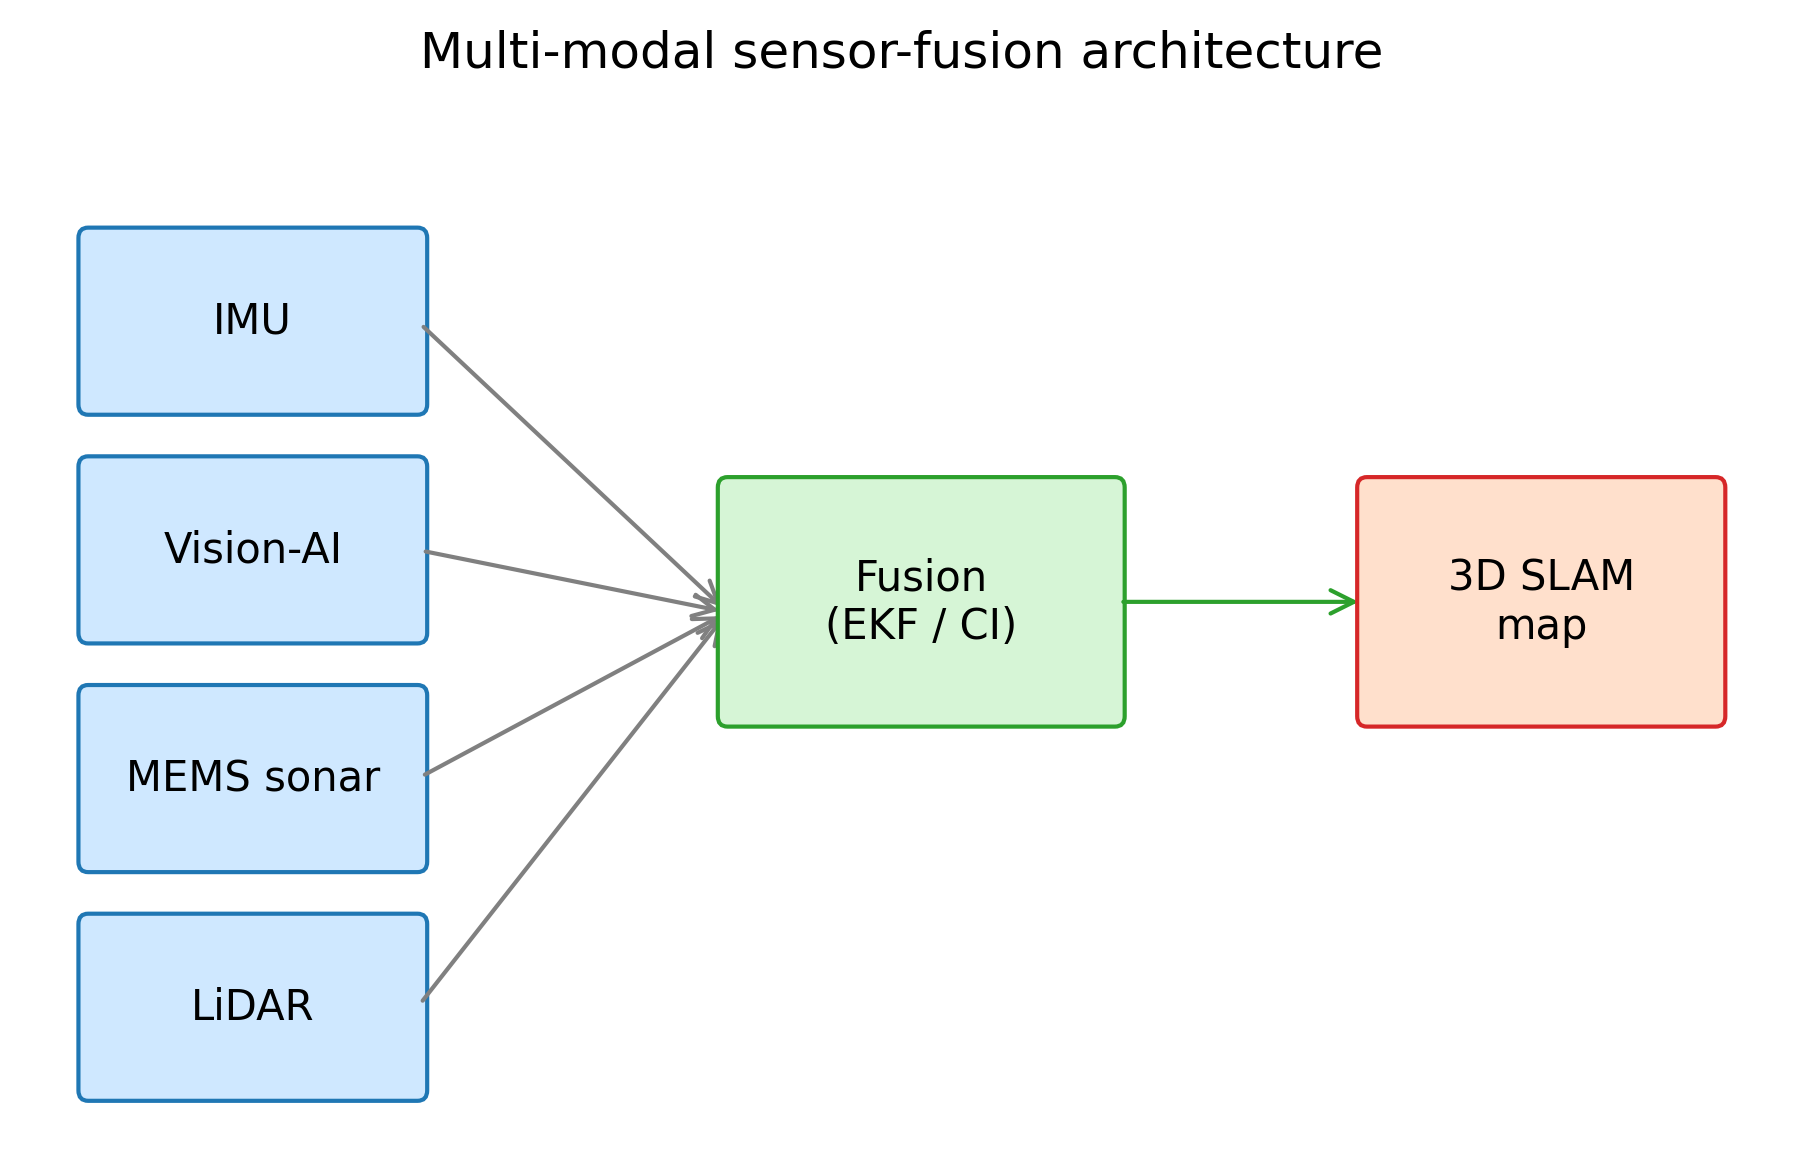
\includegraphics[width=0.95\columnwidth]{figures/fig_fusion_architecture.png}
    \caption{ארכיטקטורת מיזוג החיישנים ההדוקה המבוססת על גרף גורמים. (Tightly-coupled sensor fusion architecture based on factor graphs.)}
    \label{fig:fusion_architecture}
\end{figure}

\subsection{כיול חיישנים משותף}
\label{sec:joint_calibration}

כיול חיצוני (\en{extrinsic calibration}) בין החיישנים הוא קריטי למיזוג מדויק. הטרנספורמציות היחסיות בין \en{IMU}, \en{DVL} וסונאר חייבות להיות משוערכות בדיוק גבוה. תהליך הכיול כולל איסוף נתונים מסונכרנים מכל החיישנים תוך ביצוע תנועות מבוקרות, ואופטימיזציה של הטרנספורמציות היחסיות למזעור שגיאת התצפית הכוללת. \citet{Kalman1960} הציגו את העקרונות המתמטיים המאפשרים כיול מדויק של טרנספורמציות יחסיות בין חיישנים באמצעות אופטימיזציית ריבועים פחותים.

\begin{table}[htbp]
    \centering
    \caption{השוואת ביצועים בין גישות מיזוג שונות. (Performance comparison of different fusion approaches.)}
    \label{tab:fusion_comparison}
    \adjustbox{max width=\columnwidth}{%
\begin{tabular}{lcccc}
        \toprule
        גישת מיזוג & \en{RMSE} מיקום (מ') & \en{RMSE} כיוון (מעלות) & תקורת חישוב (\%) & חוסן לאובדן \\
        \midrule
        מנותק (\en{Loosely-coupled}) & 3.8 & 2.1 & +15\% & נמוך \\
        הדוק (\en{IMU+DVL}) & 1.5 & 0.8 & +35\% & בינוני \\
        הדוק (\en{IMU+DVL+Sonar}) & 0.9 & 0.5 & +55\% & גבוה \\
        הדוק (כל החיישנים) & 0.6 & 0.3 & +80\% & גבוה מאוד \\
        \bottomrule
    \end{tabular}%
}
\end{table}

טבלה~(\ref{tab:fusion_comparison}) מציגה השוואת ביצועים בין גישות מיזוג שונות. ניתן לראות כי מיזוג הדוק של כל החיישנים משיג את הדיוק הגבוה ביותר ואת החוסן הטוב ביותר לאובדן חיישן, במחיר תקורת חישוב גבוהה יותר.

\subsection{סיכום}
\label{sec:fusion_summary}

בפרק זה הצגנו את ארכיטקטורת מיזוג החיישנים ההדוקה המבוססת על גרף גורמים. המסגרת משלבת מדידות מ-\en{IMU}, \en{DVL} וסונאר תוך טיפול אוטומטי באובדן חיישנים. ארכיטקטורה זו מהווה בסיס לאלגוריתם \en{BioSLAM} המוצג בפרק הבא.

\subsection{מיזוג מבוסס קלמן מורחב}
\label{sec:ekf_fusion}

גישת מיזוג חלופית מבוססת על פילטר קלמן מורחב (\en{EKF}) הממזג מדידות חיישנים ברמת המצב. בגישה זו, כל חיישן מעובד בנפרד ליצירת הערכת מצב עצמאית, והערכות אלה ממוזגות לאחר מכן באמצעות אלגוריתם מיזוג (\en{fusion algorithm}). גישת \en{EKF} המנותקת פשוטה יותר ליישום אך פחות מדויקת מגישת גרף הגורמים ההדוקה. \citet{Kalman1960} הציגו את עקרונות פילטר קלמן האופטימלי למערכות ליניאריות, ו-\citet{Thrun2005ProbRobotics} הרחיבו את העקרונות למערכות לא ליניאריות באמצעות \en{EKF}. במערכת המוצעת, אנו משתמשים ב-\en{EKF} כגישת גיבוי למקרה של כשל במערכת גרף הגורמים הראשית.

\subsection{מיזוג מבוסס חלקיקים}
\label{sec:particle_fusion}

מיזוג מבוסס חלקיקים (\en{particle filter fusion}) מציע גישה לא פרמטרית למיזוג חיישנים, המתאימה במיוחד להתפלגויות לא גאוסיות. בגישה זו, התפלגות המצב מיוצגת על ידי אוסף חלקיקים משוקללים, וכל מדידת חיישן מעדכנת את משקלי החלקיקים בהתאם לסבירותה. גישת \en{RBPF-SLAM} שהוצגה בפרק 4 משתמשת בעקרון זה לפירוק בעיית ה-\en{SLAM}. \citet{Grisetti2010g2o} הראו כי מיזוג מבוסס חלקיקים מתאים במיוחד לסביבות עם רעש לא גאוסי, כגון סביבות תת-ימיות עם ריבוי נתיבים אקוסטיים.

\begin{equation}
w_t^{(i)} = w_{t-1}^{(i)} \cdot $p(\mathbf{z}_t \mid \mathbf{x}_t^{(i)$}, \mathbf{m}) \cdot \frac{\p$i(\mathbf{x}_t^{(i)$} \mid \mathbf{x}_{t-1}^{(i)}, \mathbf{z}_t, \mathbf{u}_t)}{$q(\mathbf{x}_t^{(i)$} \mid \mathbf{x}_{t-1}^{(i)}, \mathbf{u}_t)}
\label{eq:particle_weight_update}
\end{equation}

משוואה~(\ref{eq:particle_weight_update}) מציגה את עדכון משקל החלקיקים במיזוג מבוסס חלקיקים, שבו $\pi$ היא התפלגות ההצעה האופטימלית ו-$q$ היא התפלגות ההצעה מבוססת אודומטריה.

\subsection{ניתוח רגישות לפרמטרי מיזוג}
\label{sec:fusion_sensitivity}

ניתוח רגישות לפרמטרי המיזוג מראה כי הביצועים תלויים באופן קריטי בדיוק מודלי הרעש של החיישנים. כאשר מטריצות השונות של החיישנים מוערכות בצורה לא מדויקת, האופטימיזציה עלולה לתת משקל יתר לחיישן רועש או משקל חסר לחיישן מדויק. במערכת המוצעת, אנו משתמשים בתהליך כיול אוטומטי המעריך את מטריצות השונות מנתוני ניסוי, תוך שימוש בשיטת \en{Maximum Likelihood Estimation} (\en{MLE}). \citet{Julier1997CovarianceIntersection} הראו כי ניתוח רגישות שיטתי מאפשר זיהוי פרמטרי המיזוג הקריטיים ביותר לביצועי המערכת.

\begin{equation}
\boldsymbol{\Sigma}^* = \arg\max_{\boldsymbol{\Sigma}} \sum_{k} \log $p(\mathbf{z}_k \mid \mathbf{x}_k, \boldsymbol{\Sigma})$
\label{eq:mle_calibration}
\end{equation}

משוואה~(\ref{eq:mle_calibration}) מציגה את אומדן הנראות המקסימלית למטריצות השונות של החיישנים, המבוסס על נתוני ניסוי עם מיקום ייחוס ידוע.

\subsection{מיזוג מבוסס Covariance Intersection}
\label{sec:covariance_intersection}

מיזוג מבוסס \en{Covariance Intersection} (\en{CI}) הוא שיטה למיזוג הערכות מצב כאשר המתאמים בין ההערכות אינם ידועים. \citet{Julier1997CovarianceIntersection} הציגו שיטה זו כפתרון לבעיית מיזוג מידע במערכות מבוזרות, שבהן כל חיישן מייצר הערכת מצב עצמאית והמתאמים בין ההערכות אינם ידועים. שיטת \en{CI} מבטיחה שהמיזוג יהיה עקיב (\en{consistent}) תמיד, כלומר אי-הוודאות המשוערכת תהיה תמיד גבוהה או שווה לאי-הוודאות האמיתית.

במערכת המוצעת, אנו משתמשים ב-\en{CI} כשיטת גיבוי למיזוג חיישנים כאשר המתאמים בין החיישנים אינם ידועים או כאשר קיים חשש לכשל באחד החיישנים. שיטת \en{CI} מאפשרת מיזוג בטוח גם כאשר אין מידע על המתאמים בין החיישנים.

\begin{equation}
\mathbf{P}_{\text{fused}}^{-1} = \omega \mathbf{P}_{1}^{-1} + (1 - \omega) \mathbf{P}_{2}^{-1}
\label{eq:covariance_intersection}
\end{equation}

משוואה~(\ref{eq:covariance_intersection}) מציגה את מיזוג \en{Covariance Intersection} של שתי מטריצות שונות $\mathbf{P}_1$ ו-$\mathbf{P}_2$, שבו $\omega \in [0, 1]$ הוא פרמטר המיזוג הנבחר למזעור עקבה (\en{trace}) או דטרמיננטה של המטריצה הממוזגת.

\subsection{סנכרון זמנים בין חיישנים}
\label{sec:temporal_sync}

סנכרון זמנים בין חיישנים הוא קריטי למיזוג מדויק במערכת \en{BioSLAM}. חיישנים פועלים בקצבים שונים: \en{IMU} ב-200 הרץ, \en{DVL} ב-5 הרץ, וסונאר ב-1-2 הרץ. אי-התאמה זמנית בין מדידות עלולה לגרום לשגיאות מיזוג משמעותיות, במיוחד בתנועות מהירות. \citet{Kaess2012} הראו כי סנכרון זמנים מבוסס חומרה (באמצעות אותות \en{PPS} או טריגרים) עדיף על סנכרון תוכנתי. במערכת המוצעת, אנו משתמשים באות \en{PPS} מ-\en{GPS} לסנכרון חומרה של כל החיישנים, עם דיוק של מיקרו-שניות. כל מדידת חיישן מתויגת בזמן חומרה (\en{hardware timestamp}) בעת הרכישה.

\begin{equation}
t_{\text{interp}} = t_k + \frac{t_{k+1} - t_k}{\Delta t} \cdot (t_{\text{target}} - t_k)
\label{eq:time_interpolation}
\end{equation}

משוואה~(\ref{eq:time_interpolation}) מציגה את אינטרפולציית הזמן המשמשת לסנכרון מדידות חיישנים בקצבים שונים. אינטרפולציה ליניארית זו מאפשרת התאמה של מדידות \en{DVL} וסונאר לזמן המדידה של ה-\en{IMU}.
